\documentclass[12pt,oneside]{article}
\usepackage{makeidx,anysize,mflogo,xspace,float,epsfig,url}
\usepackage{amsmath,amsfonts,amssymb,a4wide} 
\usepackage[utf8]{inputenc}
%\usepackage[francais]{babel}
%\usepackage[french]{babel}
\urlstyle{sf}
%\usepackage{subcaption}
\usepackage{hyperref}
\usepackage{graphicx}
\usepackage{graphics}
\usepackage{float}
\usepackage{caption}
\usepackage{colordvi} %??
\usepackage{listings} 
\usepackage{subfigure}
\usepackage{subfloat}
\usepackage{xcolor}
\graphicspath{{./figures/}}
%\usepackage[labelsep=quad,indention=10pt]{subfig}
\definecolor{grey}{rgb}{0.95,0.95,0.95} % on définit la couleur grise
	% (c'est un gris très clair)
	\definecolor{red}{rgb}{1.0,0.0,0.0} 
	\definecolor{green}{rgb}{0.0,0.8,0.0}
	\definecolor{blue}{rgb}{0.0,0.0,1.0}
	\lstloadlanguages{bash,Java,C,C++,csh,make,sh}%%[Visual]Basic,xml}
	\lstset{frame=none,basicstyle=\footnotesize,breaklines,tabsize=2,captionpos=b,
		prebreak={\hbox{$\rightarrow$}},postbreak={\hbox{$\hookrightarrow$}},
		showstringspaces=false,backgroundcolor=\color{grey}\bfseries,
		keywordstyle=\color{blue},commentstyle=\color{green}\textit,
		stringstyle=\color{red}\ttfamily,abovecaptionskip=2pt,aboveskip=0pt,
		belowskip=0pt,belowcaptionskip=0pt,numbers=none,columns=fullflexible, backgroundcolor=\color{grey}}
%left,numberstyle=\footnotesize,
%		stepnumber=2,numbersep=1pt}

\begin{document}


\begin{center}
{\bf \Large Redpitaya: third example} \\ \ \\
G. Goavec-M\'erou, J.-M Friedt \\ \ \\ \today
\end{center}

This tutorial is a sequel to the previous one on which it is based. In addition to 
copying the ADC input to the DAC output, we wish to add to the stream of data sent
to the user (PS) a filtered copy of one of the ADC inputs. The Finite Impulse Response
(FIR) filter will process the 125~MS/s stream with integer coefficients configured from
userspace (PS) (Fig. \ref{fin}). Furthermore, we wish to extend capability beyond a single
complex stream: we will now stream two parallel real data, which could be extended to more than
two channels.

\begin{figure}[h!tb]
\hspace{-2cm}
%\begin{center}
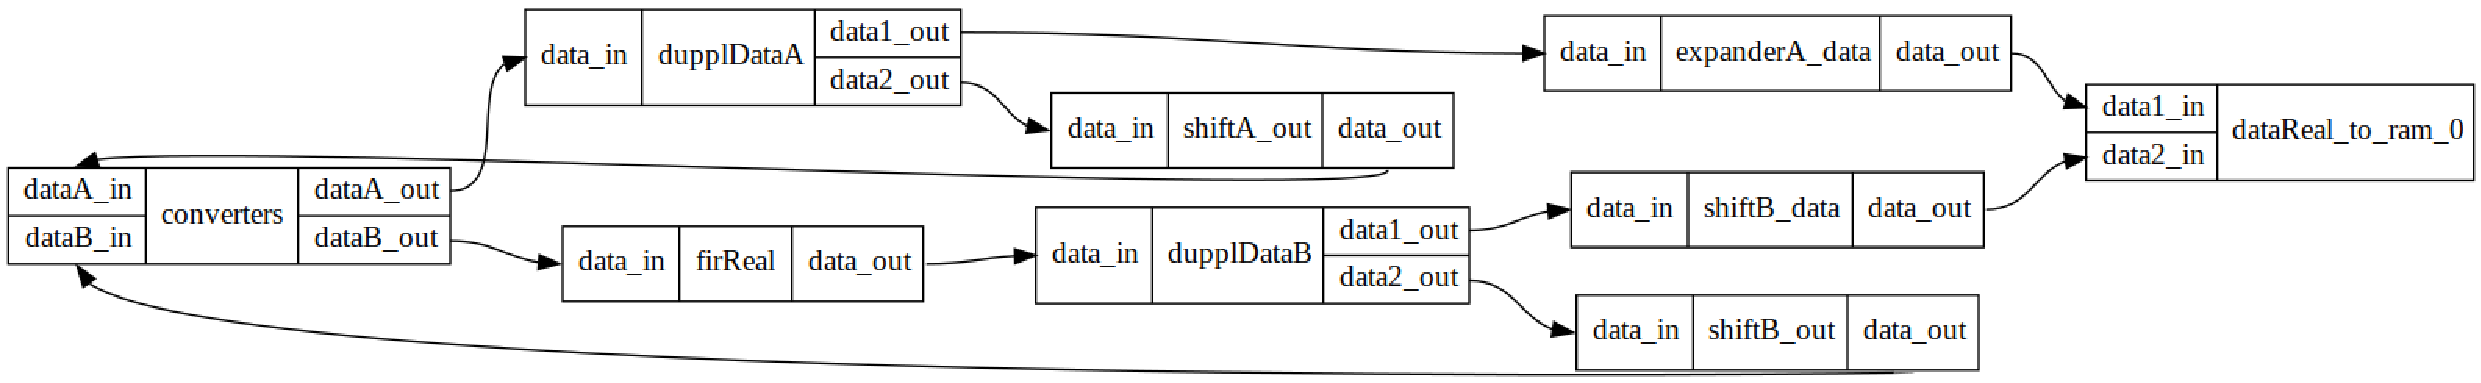
\includegraphics[width=1.2\textwidth]{figures/structs.pdf}
%\end{center}

\hspace*{-1.5cm}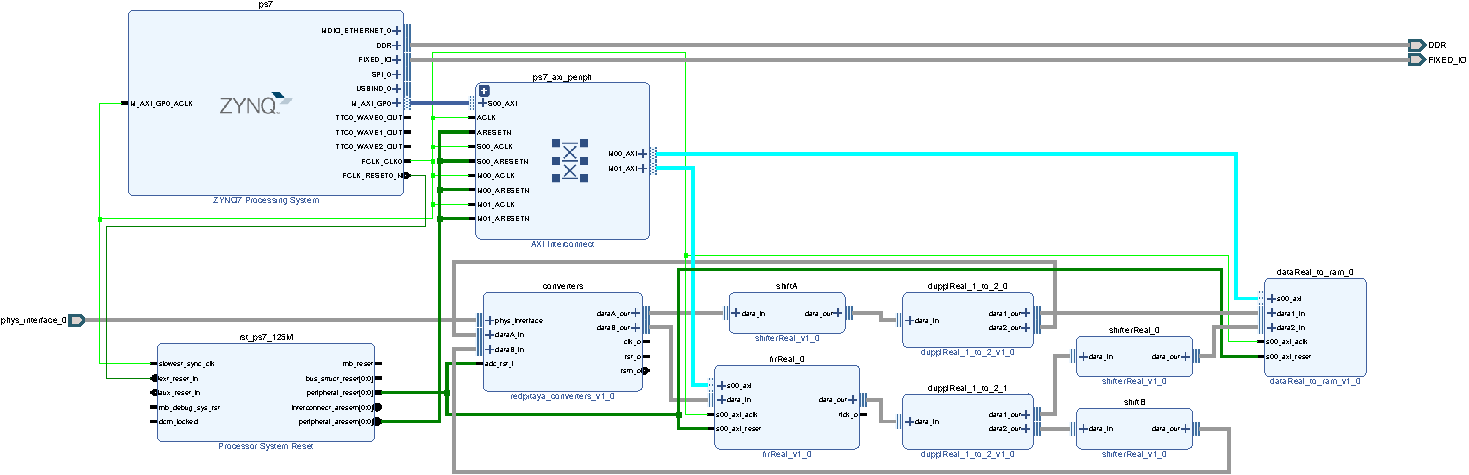
\includegraphics[width=1.2\linewidth]{combinedADC_DAC_data2ram_FIR.pdf}
\caption{Schematic of the objective and final processing chain described in this document}
\label{fin}
\end{figure}

\section{FIR configuration}

The ADC to DAC and ADC to RAM blocks are the same as before, with stream
dupplication every time a new datastream must reach two users. The novely
is now the use of a FIR filter, whose input width the match the incoming
datastream width.

%JMF : verifier Data Width
Double click on the FIR block and update the Data Width ({\tt Data In Size}) to 14~bits (or 16-bits for
the 16-bit Redpitaya). The input data width (in bits) is called $P$.

The coefficient width $M$ ({\tt COEFF Size}) will define the size of the data transferred from the PS
to the PL, as stored as a column of decimal values written in human readable ASCII
format. The number of coefficients $N$ ({\tt Nb COEFF}) and number of bits defining each coefficient are
defined at synthesis time and must match the largest expected filter (as well as
available resources).

Theoretically, $Q=P+M+\log_2(N)$ bits are generated at the output of the FIR convolution.
Practically, this number of bits is grossly over-estimated, and truncation can be 
considered based on the knowledge of the coefficients defining the FIR. Taking the
$\log_2$ of the sum of the absolute values of the coefficients will give a much more 
conservative number of bits relevant at the output. While all internal computations are
performed on $Q$ bits, the output can be {\em truncated} to the {\em lower}
Output Size bits ({\tt Data Out Size}).
% JMF : verifier Output Size

The default behaviour of the FIR filter is to decimate the output: doing so, only useful
outputs will be computed, saving computational resources in the FPGA. In the TCL example
in the {\tt design} directory, the decimation factor is {\tt DECIMATE\_FACTOR 5} so that
the output feeding the DAC output is ``only'' clocked at 25~MS/s.

The user might then decide to shift to the right the result to drop some of the 
least-significant bits, as illustrated here with the selection of outputting 16~bits
from the FIR filter (e.g. for further computations in the PL) and shifting the 2 least
significant bits to send 14-bit wide words (as expected from the legacy Redpitaya ADC 
datastream -- 16 bits for the 16-bit Redpitaya) to the PS.

To summarize:
\begin{itemize}
\item disconnect interface between {\tt converters/dataB\_out} and {\tt dupplDataB/data\_in};
\item add {\tt firReal} IP, renamed as {\tt fir00} with:
\begin{itemize}
\item {\tt DATA\_IN\_SIZE}: 14;
\item {\tt DATA\_OUT\_SIZE}: 19;
\item {\tt NB\_COEFF}: 32;
\item {\tt DECIMATE\_FACTOR}: 5;
\end{itemize} 
\item update dupplDataB with {\tt DATA\_SIZE} = 19
\item suppress {\tt convertRealToCplx} and {\tt data1600};
\item add {\tt dataReal\_to\_ram} IP, renamed as {\tt data1600}, with:
\begin{itemize}
\item {\tt DATA\_SIZE} = 16;
\item {\tt NB\_SAMPLE} = 4096;
\item {\tt NB\_INPUT} = 2;
\end{itemize}
\item add {\tt expanderReal} IP, connect this block between {\tt dupplDataA} and
{\tt data1600/data1\_in} with:
\begin{itemize}
\item {\tt DATA\_IN\_SIZE} = 14;
\item {\tt DATA\_OUT\_SIZE} = 16;
\end{itemize}
\item add {\tt shifterReal} IP, connect this block between {\tt dupplDataB} and
{\tt data1600/data2\_in} with:
\begin{itemize}
\item {\tt DATA\_IN\_SIZE} = 19;
\item {\tt DATA\_OUT\_SIZE} = 16;
\end{itemize}
\end{itemize}

\section{PS: Linux kernel driver}

Rather than using a single complex stream to communicate with the PS, we have now
selected the {\tt dataReal\_to\_ram} to define multiple real streams. The driver
is the same than {\tt dataComplex\_to\_ram}, so that this part of the XML
may be left unchanged (memory address must be checked, as shown for example
on Fig. \ref{addr}), in 
addition to which we wish to communicate with the FIR to define the coefficients. 
This time, the {\tt module\_generator} XML configuration file should look like

\lstinputlisting[language=xml]{./module_generator.xml}

%\begin{verbatim}
%<?xml version="1.0" encoding="utf-8"?>
%<drivers name="project_1" version="1.0">
%	<driver name ="data16_multi_to_ram" >
%		<board_driver name="data1600" id = "0"
%			base_addr="0x43c00000" addr_size="0xffff" />
%	</driver>
%	<driver name ="fir16bits" >
%		<board_driver name="datafir0" id = "0"
%			base_addr="0x43c10000" addr_size="0xffff" />
%	</driver>
%</drivers>
%\end{verbatim}

\begin{figure}[h!tb]
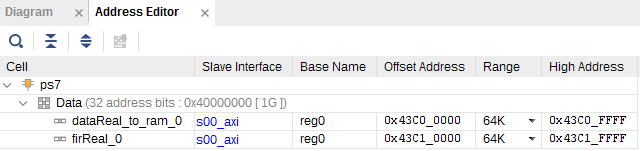
\includegraphics[width=\linewidth]{address}
\caption{Address range used by the IPs as defined by Vivado.}
\label{addr}
\end{figure}

\section{On the Redpitaya ...}

For communicating with the FIR, we will benefit from an existing library function as
implemented in {\tt liboscimp\_fpga} (see \$OSCIMP\_DIGITAL\_LIB).
This library must be installed by:
\begin{verbatim}
make && make install
\end{verbatim}
to place the .so in {\tt buildroot} {\tt target} dir (the board must be flashed again),
or by
\begin{verbatim}
make && make install_ssh
\end{verbatim}
to transfer the .so to the embedded board's {\tt /usr/lib} directory by using {\tt
ssh}.
By default target IP is 192.168.0.10, which can be updated to match another
network configuration with
\begin{verbatim}
make && IP=AA.BB.CC.DD.EE make install_ssh
\end{verbatim}

\lstinputlisting[language=C]{./app/main.c}

Examples of outputs of running this program are given in Figs. \ref{fir1} and
\ref{fir2}: all filter
lengths are set to 32, with a varying number of non-null values set to 1 in the beginning
of the filter. Since in this design the FIR output is routed to the DAC, an oscilloscope is
first used to monitor the generated signal frequency and the filtered signal amplitude
(oscilloscope ``Measure'' functions set to ``Frequency C1'' and ``Peak to Peak Amplitude C3'').
In all cases the generated signal is 1.5~V$_{pp}$.

The transfer function of a FIR filter is the Fourier transform of its coefficients so that
the transfer function of rectangular window FIR filters are sinc functions. The expected
transfer functions are displayed in Fig. \ref{fir1} (top) and the experiemental amplitude
of the FIR output for varying filter window width and notch frequency are shown in Fig.
\ref{fir1} (bottom). The notch frequency are in excellent agreement, the amplitude 
measurements are plagued by poor resolution of the oscilloscope measurement.

\begin{figure}[h!tb]
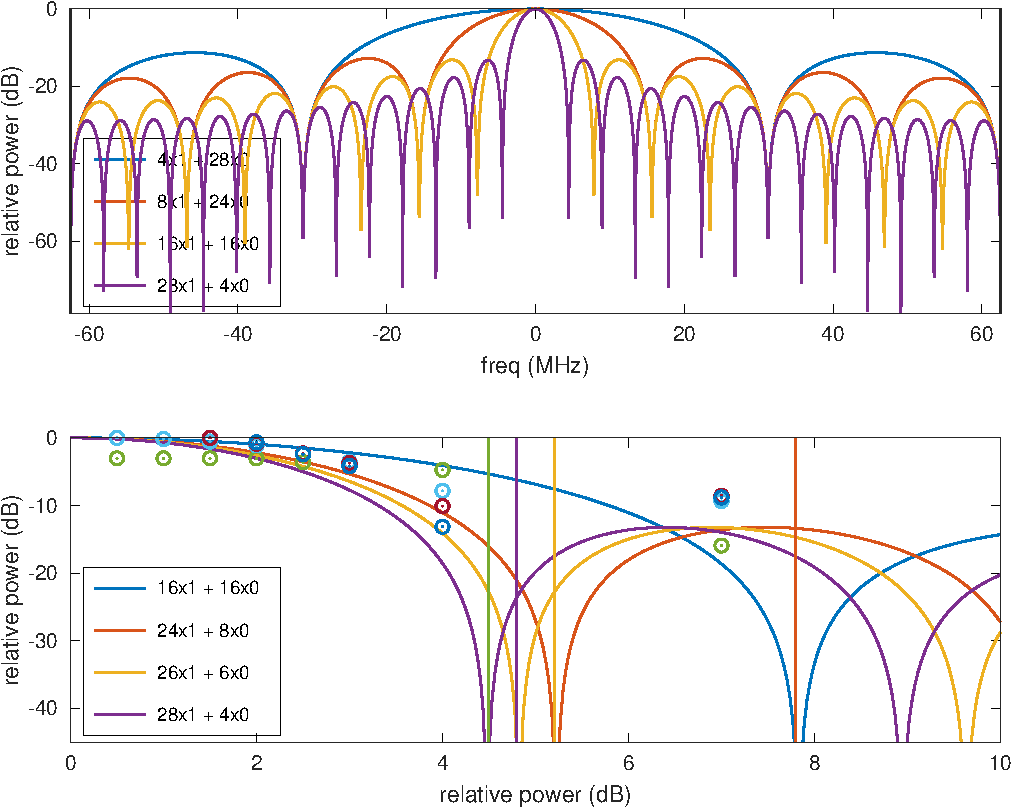
\includegraphics[width=.68\linewidth]{results/model.pdf}
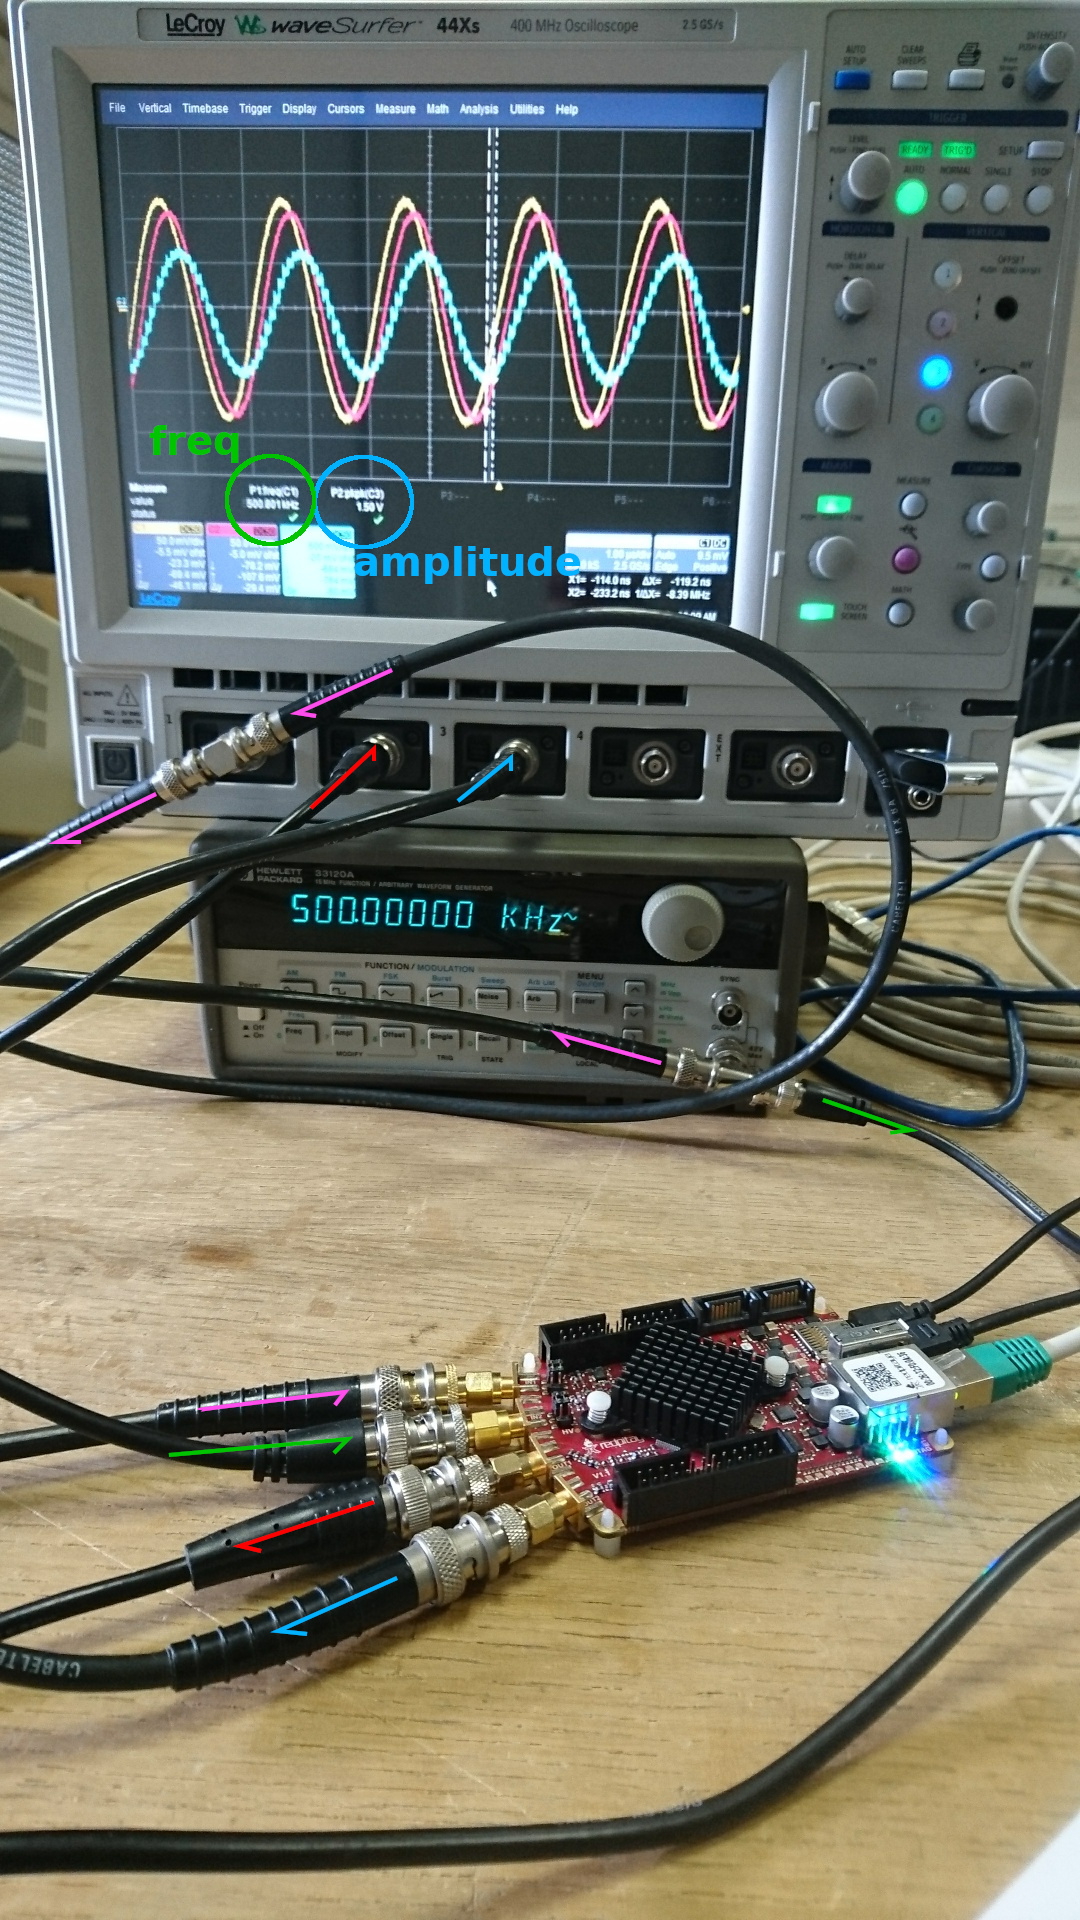
\includegraphics[width=.31\linewidth]{results/DSC_0368_3ann.JPG}
\caption{Left: transfer function of rectangular FIR windows (top) and measured amplitude and notch
frequencies (bottom). On the bottom chart, vertical lines are located at the observed notch
frequency. Right: experimental setup, including arrows showing that the same driving signal
is feeding both ADCs, and the two DAC outputs are either copies of one ADC or the filtered output
of the other ADC.}
\label{fir1}
\end{figure}

Beyond these oscilloscope measurements, datasets can be dumped from the {\tt data\_to\_ram}
for further processing. Various
test FIRs are designed by clearnig to 0 all coefficients except the first ones, which 
might be either set to 1 for the first 16 coefficients, or set to 4 for the first 4 coefficients 
(keeping the total power constant). Since sampling is at 125~MS/s, the cutoff frequency
of a 16-tap long coefficient must be about 7.8~MHz: most of the recorded datasets
(1 or 6~MHz) are not affected by the filter except for the bottom one in which the
signal frequency becomes close to the cutoff frequency of the filter. The group delay 
(time needed between filling input and providing the first output) is observed as the
phase shift between input and output (Fig. \ref{fir2})

\begin{figure}[h!tb]
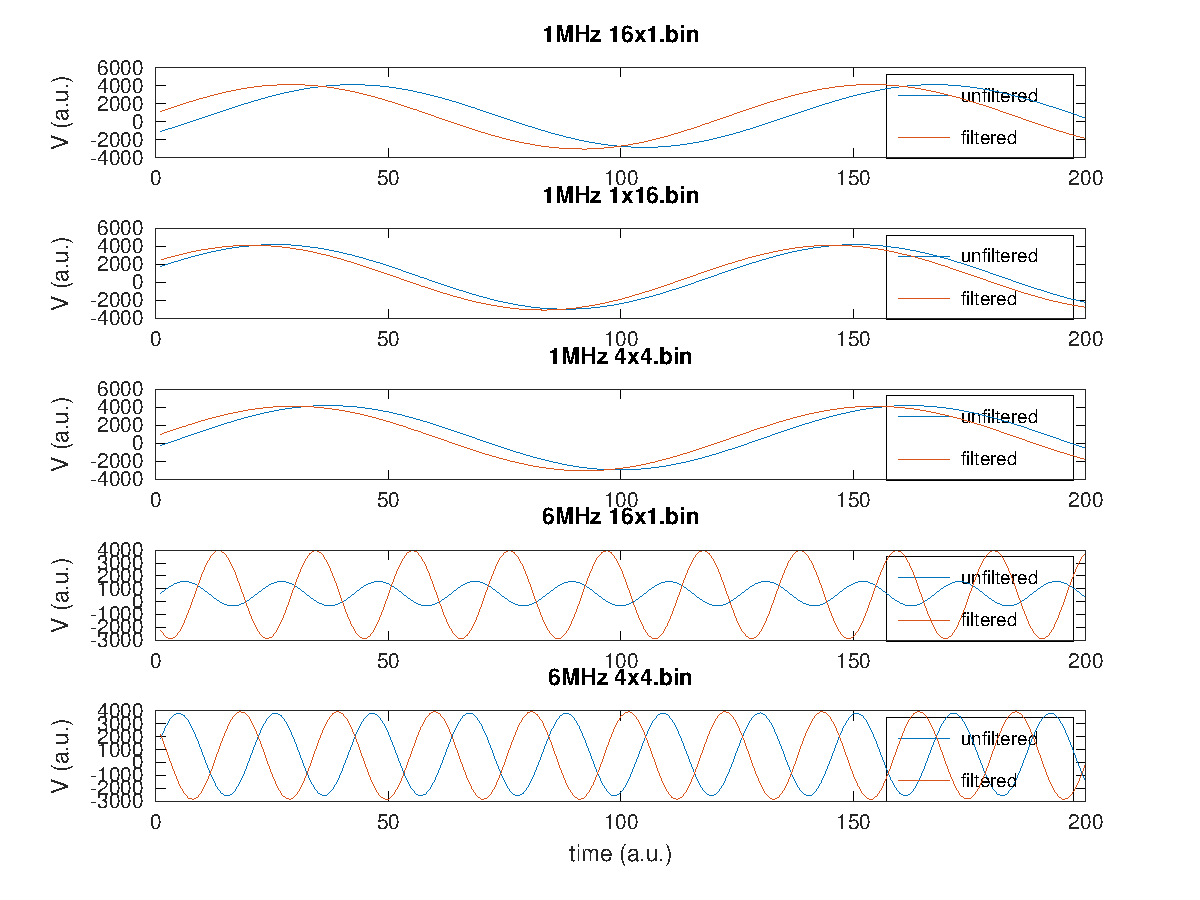
\includegraphics[width=\linewidth]{figures/mesures}
\caption{Filtered output (blue) with respect ot the input (red) driving signal:
{\tt data\_to\_ram} outputs.}
\label{fir2}
\end{figure}

Collecting the filtered output on the {\tt data\_to\_ram} device demonstrates how the
FPGA can be efficiently used either to process the stream straight from the acquisition
interface through the various processing blocks, or as co-processor from data provided
by the CPU and running through the FPGA before being recovered by the CPU.
\end{document}
% 
% cp ./project_1.runs/impl_1/design_1_wrapper.bit .
% bootgen -image design_1_wrapper.bif -arch zynq -process_bitstream bin
% 
% jmfriedt@rugged:~/xilinx/oimp/doc/tutorials/4-fpga_FIR/project_1/app$ /home/jmfriedt/enseignement/ufr/platforms/redpitaya/buildroot-2018.08.1/output/build/linux-3f3c7b60919d56119a68813998d3005bca501a40/scripts/dtc/dtc -@ -I dts -O dtb -o project_1.dtbo project_1.dts
% 
%  source /home/jmfriedt/xilinx/oimp/fpga_driver/sourceme.ggm 
%  export BOARD_NAME=redpitaya
%  export BR_DIR=/home/jmfriedt/enseignement/ufr/platforms/redpitaya/buildroot-2018.08.1/
%  make
% 
% 
% /home/jmfriedt/enseignement/ufr/platforms/redpitaya/buildroot-2018.08.1/output/host/usr/bin/arm-linux-gcc -I /home/jmfriedt/xilinx/oimp/fpga_lib -o ma_lecture ma_lecture.c -L/home/jmfriedt/xilinx/oimp/fpga_lib -loscimp_fpga
